\documentclass{standalone}

%\url{}
\usepackage{tikz}
\usepackage{comment}
\usepackage{bm}


%%%%%%%%%%%%%%%%%%%%%%%%%%%%%%%%%%%%%%%%%%%%%%%%


\makeatletter
\def\grd@save@target#1{%
  \def\grd@target{#1}}
\def\grd@save@start#1{%
  \def\grd@start{#1}}
\tikzset{
  grid with coordinates/.style={
    to path={%
      \pgfextra{%
        \edef\grd@@target{(\tikztotarget)}%
        \tikz@scan@one@point\grd@save@target\grd@@target\relax
        \edef\grd@@start{(\tikztostart)}%
        \tikz@scan@one@point\grd@save@start\grd@@start\relax
        \draw[minor help lines] (\tikztostart) grid (\tikztotarget);
        \draw[major help lines] (\tikztostart) grid (\tikztotarget);
        \grd@start
        \pgfmathsetmacro{\grd@xa}{\the\pgf@x/1cm}
        \pgfmathsetmacro{\grd@ya}{\the\pgf@y/1cm}
        \grd@target
        \pgfmathsetmacro{\grd@xb}{\the\pgf@x/1cm}
        \pgfmathsetmacro{\grd@yb}{\the\pgf@y/1cm}
        \pgfmathsetmacro{\grd@xc}{\grd@xa + \pgfkeysvalueof{/tikz/grid with coordinates/major step}}
        \pgfmathsetmacro{\grd@yc}{\grd@ya + \pgfkeysvalueof{/tikz/grid with coordinates/major step}}
        \foreach \x in {\grd@xa,\grd@xc,...,\grd@xb}
        \node[anchor=north] at (\x,\grd@ya) {\pgfmathprintnumber{\x}};
        \foreach \y in {\grd@ya,\grd@yc,...,\grd@yb}
        \node[anchor=east] at (\grd@xa,\y) {\pgfmathprintnumber{\y}};
      }
    }
  },
  minor help lines/.style={
    help lines,
    step=\pgfkeysvalueof{/tikz/grid with coordinates/minor step}
  },
  major help lines/.style={
    help lines,
    line width=\pgfkeysvalueof{/tikz/grid with coordinates/major line width},
    step=\pgfkeysvalueof{/tikz/grid with coordinates/major step}
  },
  grid with coordinates/.cd,
  minor step/.initial=.2,
  major step/.initial=1,
  major line width/.initial=2pt,
}

\makeatother
\begin{document}
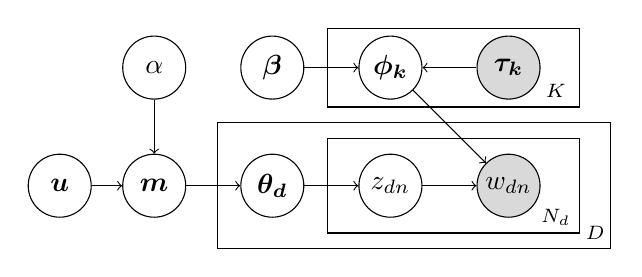
\begin{tikzpicture}
%%%%%%%%%%%%%%%%%%%%%%%%%%%%%%%%%%%%%%%%%%%%%%%%
%%%%%coordination system below
\begin{comment}
\draw[help lines,step=.2] (-2,-2) grid (7,4);
\draw[help lines,line width=.6pt,step=1] (-2,-2) grid (7,4);
\foreach \x in {-2,-1,0,1,2,3,4,5,6,7}
 \node[anchor=north] at (\x,-2) {\x};
\foreach \y in {-2,-1,0,1,2,3,4}
 \node[anchor=east] at (-2,\y) {\y};
\end{comment}
%%%%%%%%%%%%%%%%%%%%%%%%%%%%%%%%%%%%%%%%%%%%%%%%
%%%%%your code below
\node (u) at (-1.2,0) [circle, draw, inner sep=0pt, minimum size=0.8cm] {\bm{$u$}};
\node (m) at (0,0) [circle, draw, inner sep=0pt, minimum size=0.8cm] {\bm{$m$}};
\node (theta) at (1.5,0) [circle, draw, inner sep=0pt, minimum size=0.8cm] {\bm{$\theta_d$}};
\node (z) at (3,0) [circle, draw, inner sep=0pt, minimum size=0.8cm] {$z_{dn}$};
\node (w) at (4.5,0) [fill=gray!30,circle, draw, inner sep=0pt, minimum size=0.8cm] {$w_{dn}$};

\node (alpha) at (0,1.5) [circle, draw, inner sep=0pt, minimum size=0.8cm] {$\alpha$};
\node (b) at (1.5,1.5) [circle, draw, inner sep=0pt, minimum size=0.8cm] {\bm{$\beta$}};
\node (phi) at (3,1.5) [circle, draw, inner sep=0pt, minimum size=0.8cm] {\bm{$\phi_k$}};
\node (tau) at (4.5,1.5) [fill=gray!30,circle, draw, inner sep=0pt, minimum size=0.8cm] {\bm{$\tau_k$}};

\draw[->] (alpha) -- (m);
\draw[->] (u) -- (m);
\draw[->] (m) -- (theta);
\draw[->] (b.east) -- (phi.west);

\draw[->] (theta.east) -- (z.west);
\draw[->] (z.east) -- (w.west);
\draw[->] (phi) -- (w);
\draw[->] (tau.west) -- (phi.east);

%D related
\draw (0.8,-.8) rectangle (5.8,.8);

%N related
\draw (2.2,-.6) rectangle (5.4,0.6);

%K related
\draw (2.2,1) rectangle (5.4,2);

\node at (5.6,-.6) {\scriptsize $D$};
\node at (5.1,-.4) {\scriptsize $N_d$};
\node at (5.1,1.2) {\scriptsize $K$};
%%%%%%%%%%%%%%%%%%%%%%%%%%%%%%%%%%%%%%%%%%%%%%%%
 
\end{tikzpicture}

\end{document}
